\begin{beginningnote}
    Si tenga presente che alcuni termini utilizzati nel documento riportano la lettera \textbf{G} in apice, allo scopo di evidenziare le parole che assumono uno specifico significato nell'ambito del progetto. Per comprenderle in maniera corretta, si rimanda il lettore al documento ``Glossario", che contiene un elenco completo di tutte le terminologie utilizzate con relative definizioni, allo scopo di costruire un linguaggio uniforme che possa migliorare la comunicazione tra i componenti interni al gruppo e gli stakeholders esterni.
\end{beginningnote}

%%%%%%%%%%%%%%%%%%%%%%%%%%%%%%%%%%%
% SCOPO DEL DOCUMENTO
%%%%%%%%%%%%%%%%%%%%%%%%%%%%%%%%%%%
\section{Scopo del documento}\label{sec:scopo_del_documento}
\par Questo documento ad uso interno del gruppo ha lo scopo di illustrare in maniera dettagliata il way of working\textsuperscript{G} adottato nell'ambito del progetto\textsuperscript{G}, descrivendo gli strumenti utilizzati, le procedure e le convenzioni adottate per la realizzazione di un prodotto che possa essere quanto più possibile di qualità e allo stato dell'arte.
\par Vista la natura del documento, è previsto che questo venga redatto in maniera incrementale, aggiornandolo man mano che il gruppo prosegue nello sviluppo del progetto ed accumula esperienza, migliorando il proprio way of working. Per una visione precisa delle modifiche, si rimanda al changelog, che descrive per ciascuna versione le differenze rispetto a quella precedente.
\par Nella realizzazione del progetto, il gruppo seguirà le linee guida dello \hyperref[sec:standard_iso/iec_12207]{standard ISO/IEC 12207}: vista la sua notorietà, l'utilizzo di questo framework rappresenta la soluzione più sicura ed affidabile. Le norme di progetto riportate nel documento saranno perciò illustrate attenendosi ai processi descritti dallo standard.

%%%%%%%%%%%%%%%%%%%%%%%%%%%%%%%%%%%
% IL PROGETTO
%%%%%%%%%%%%%%%%%%%%%%%%%%%%%%%%%%%
\section{Il progetto}\label{sec:il_progetto}
\par Il progetto nasce nell'ambito dei \textbf{sistemi gestionali di magazzino}, meglio noti con il termine inglese di \textit{Warehouse Management Systems} (WMS), con l'obiettivo di risolvere una serie di problematiche derivanti dalle soluzioni tradizionali tuttora presenti sul mercato.
\par Il focus principale sarà migliorare la user experience, tramite la realizzazione di un applicativo che proponga all'utente un'interazione con il magazzino in un ambiente di lavoro 3D: questa soluzione, rispetto ai tradizionali sistemi 2D, garantirebbe una maggiore comprensione degli spazi, proponendo una visualizzazione più intuitiva e familiare del magazzino all'utente che, di conseguenza, sarà in grado di prendere decisioni organizzative più informate ed efficienti, ottimizzando i processi di logistica.
\par Per raggiungere questo obiettivo, l'ambiente di lavoro non può essere una semplice visualizzazione del magazzino: l'utente deve poter:
\begin{itemize}
    \item Navigare l'ambiente 3D
    \item Progettare la scaffalatura e modificarla nel tempo
    \item Simulare i flussi di movimento di mezzi e prodotti
\end{itemize}
Il progetto deve concretizzarsi nella realizzazione di una web app fruibile agli impiegati d'ufficio ed incentrata sulla visualizzazione 3D del magazzino.
\par Per visionare il capitolato\textsuperscript{G} e la documentazione del gruppo, si veda la sezione \hyperref[sec:riferimenti_esterni]{Riferimenti Esterni} del documento.

\newpage
%%%%%%%%%%%%%%%%%%%%%%%%%%%%%%%%%%%
% PROCESSI PRIMARI
%%%%%%%%%%%%%%%%%%%%%%%%%%%%%%%%%%%
\section{Processi primari}\label{sec:processi_primari}

%%%%%%%%%%%%%%%%%%%%%%%%%%%%%%%%%%%
%%% FORNITURA
%%%%%%%%%%%%%%%%%%%%%%%%%%%%%%%%%%%
\subsection{Fornitura}\label{sec:processi_primari:fornitura}
Per come è definito nello standard ISO/IEC 12207, il processo di fornitura descrive tutte le attività che il fornitore deve svolgere per assicurarsi che il prodotto sia realizzato in maniera professionale e conforme alle richieste dell'acquirente. Per questa ragione, gli aspetti importanti di questa fase sono:
\begin{itemize}
    \item Determinare le risorse necessarie a completare il progetto
    \item Pianificare le procedure necessarie per completare il progetto ed assicurare un prodotto di qualità
    \item Gestire le comunicazioni con l'acquirente
\end{itemize}
\subsubsection{Determinazione di risorse e procedure}
Per sviluppare i primi due punti in maniera completa ed adeguata, il gruppo ha scelto di seguire le linee guida dello standard ed affidarsi ai processi organizzativi, il cui compito è esattamente occuparsi di tutti gli aspetti di carattere gestionale, dal punto di vista dei processi, delle infrastrutture e del personale, necessari per la realizzazione del progetto: gli output di queste fasi verranno poi utilizzati per la gestione del processo di fornitura.
\par I processi organizzativi sono descritti nella sezione \ref{sec:processi_organizzativi}, a loro dedicata.
\subsubsection{Comunicazioni con il proponente}
La corretta gestione della comunicazione con il cliente è un aspetto chiave nelle buone pratiche di ingegneria del software: agli esordi della disciplina questo punto è stato molto sottovalutato, con conseguenze gravi nel risultato finale del progetto, in particolare con il rischio che il prodotto finale non rispetti i bisogni iniziali dell'acquirente.
\par Il gruppo riconosce l'importanza di questo aspetto e si impegna a mantenere una comunicazione costante con il cliente per tutta la durata del progetto, con l'obiettivo di costruire un prodotto che soddisfi i bisogni del cliente e rispetti i requisiti prestabiliti. In particolare, le comunicazioni avverranno per:
\begin{itemize}
    \item Chiarire eventuali dubbi sul capitolato proposto
    \item Mantenersi aggiornati sui vincoli ed i requisiti che il prodotto deve rispettare
    \item Mantenersi aggiornati sullo stato di progetto
    \item Chiedere un riscontro sulla documentazione prodotta nel corso del progetto
    \item Proporre particolari soluzioni per le diverse problematiche che possono sorgere nel progetto
\end{itemize}
\par Su richiesta del cliente, la comunicazione avverrà principalmente tramite posta elettronica.
\subsubsection{Documenti da produrre}
Questo processo punta molto alla comunicazione con il cliente, per questo motivo è necessario produrre due documenti ad uso esterno, descritti di seguito, con l'obiettivo di grantire trasparenza e fornire delle metriche che permettano al cliente di comprendere meglio l'andamento del progetto nel corso del tempo.
\par Le modalità di scrittura di qualsiasi documento sono descritte nella sezione \ref{sec:processi_di_supporto:documentazione}, dedicata al processo di documentazione.
\paragraph{Piano di progetto}
Questo documento descrive la pianificazione delle attività nel corso del progetto, individuando gli obiettivi e le risorse necessarie al completamento, illustrando i dati tramite diagrammi e grafici ove possibile ed analizzando eventuali rischi che potrebbero presentarsi.
Il documento sarà diviso nelle seguenti parti:
\begin{itemize}
    \item \textbf{Analisi dei rischi}: ha lo scopo di cercare di identificare alcune difficoltà che potrebbero sorgere nel corso di progetto, proponendo delle soluzioni per mitigare queste problematiche.
    \item \textbf{Modello di sviluppo}: scelta del modello da applicare al progetto
    \item \textbf{Calendario di pianificazione}: illustra le attività da svolgere, definendo periodi e scadenze per ciascuna attività
    \item \textbf{Preventivo}: illustra l'impegno previsto per ciascuna persona e per ogni ruolo nelle diverse fasi del progetto, riepilogando i costi finali.
    \item \textbf{Consuntivo}: valutazione dei costi previsti rispetto a quelli effettivi
    \item \textbf{Mitigazione dei rischi}
\end{itemize}

\paragraph{Piano di qualifica}
Specifica le attività e procedure da seguire per assicurarsi che il codice e la documentazione prodotti nel corso del progetto siano di qualità e per assicurarsi che i processi siano svolti in maniera consona a garantire un prodotto finale allo stato dell'arte.
Il documento sarà diviso nelle seguenti parti:
\begin{itemize}
    \item \textbf{Qualità di processo}: specifica le attività e metriche da adottare per assicurare un controllo sulla qualità dei processi
    \item \textbf{Qualità di prodotto}: specifica le attività e metriche da adottare per assicurare un controllo sulla qualità dei prodotti
    \item \textbf{Test}: specifice quali test effettuare per garantire conformità con i requisiti prestabiliti
    \item \textbf{Resoconto}: retrospettiva dell'attività di verifica con eventuali proposte di miglioramento.
\end{itemize}

\subsubsection{Strumenti}
\paragraph{Microsoft Excel}
Si tratta del programma più utilizzato per la produzione e gestione di fogli elettronici: offre funzionalità particolarmente avanzate, in particolare il gruppo ha scelto di usarlo perché permette la costruzione di grafici a partire dai dati inseriti nelle celle del foglio elettronico.
\par Lo strumento è reperibile al sito:
\begin{center}
    \url{https://www.microsoft.com/it-it/microsoft-365/excel}
\end{center}

\paragraph{Microsoft Project}
È un software per il project management che permette di descrivere la pianificazione di progetto tramite l'utilizzo di diagrammi di Gantt, che garantiscono migliore organizzazione tramite una visione più efficace delle attività nel corso del tempo e permettono un tracciamento migliore, visualizzando anche le dipendenze fra attività.
\par Lo strumento è reperibile al sito:
\begin{center}
    \url{https://www.microsoft.com/it-it/microsoft-365/project/project-management-software}
\end{center}


%%%%%%%%%%%%%%%%%%%%%%%%%%%%%%%%%%%
%%% SVILUPPO
%%%%%%%%%%%%%%%%%%%%%%%%%%%%%%%%%%%
\subsection{Sviluppo}\label{sec:processi_primari:sviluppo}

\begin{center}
    \color{red}*** TODO ***
\end{center}

\newpage
%%%%%%%%%%%%%%%%%%%%%%%%%%%%%%%%%%%
% PROCESSI DI SUPPORTO
%%%%%%%%%%%%%%%%%%%%%%%%%%%%%%%%%%%
\section{Processi di supporto}\label{sec:processi_di_supporto}

%%%%%%%%%%%%%%%%%%%%%%%%%%%%%%%%%%%
%%% DOCUMENTAZIONE
%%%%%%%%%%%%%%%%%%%%%%%%%%%%%%%%%%%
\subsection{Documentazione}\label{sec:processi_di_supporto:documentazione}
La documentazione assume un ruolo fondamentale per la buona riuscita di un progetto e, se realizzata in maniera professionale, contribuisce alla realizzazione di un prodotto di qualità:
\begin{itemize}
    \item Permette di costruire uno storico del progetto, tenendo traccia del suo andamento dall'inizio alla fine e motivando le scelte che sono state fatte nel percorso.
    \item Rappresenta un metodo di comunicazione affidabile non solo tra il gruppo e gli stakeholders esterni, ma anche tra membri interni del gruppo, potenziando la collaborazione.
    \item Migliora la manutenzione del prodotto e permette ad esterni di comprenderne meglio il funzionamento, infatti una delle principali cause di abbandono di un progetto software è dovuta alla scarsa documentazione.
\end{itemize}
Risulta quindi evidente la necessità di stabilire un metodo rigoroso ed efficace per la redazione dei documenti, al fine di sfruttarne al massimo le potenzialità.
\subsubsection{Uso di un documento}
I documenti prodotti nel corso del progetto non hanno tutti uno stesso uso. Il gruppo fa distinzione tra:
\begin{itemize}
    \item Documenti interni: sono documenti per il solo uso interno del gruppo e non necessari agli stakeholders esterni. Di questa categoria fanno parte i verbali degli incontri tra membri del gruppo e il documento ``Norme di Progetto".
    \item Documenti esterni: sono documenti prodotti per gli stakeholders esterni (l'azienda proponente e il committente), che devono poterli visionare, scegliendo se approvarli o rifiutarli.
\end{itemize}
\subsubsection{Ciclo di vita del documento}
La documentazione prodotta durante un progetto di ingegneria software è estremamente legata al codice e alle versioni di rilascio del prodotto, per cui è necessario descrivere il ciclo di vita del documento con una struttura ciclica: ciascun documento, infatti, evolve nel corso del progetto a seconda di come cambiano i requisiti e le necessità del prodotto e non è da considerarsi monouso.
Il gruppo ha scelto di definire il ciclo di vita del prodotto nel seguente modo:
\begin{itemize}
    \item La produzione del documento ha origine dal bisogno di mettere per iscritto delle informazioni necessarie al progetto
    \item Il documento entra in fase di redazione e viene scritto
    \item Una volta completato, il documento passa alla fase di verifica, nella quale ci si accerta che il documento sia prodotto secondo le regole prestabilite: se così non fosse, il documento dovrà essere corretto prima di passare alla prossima fase
    \item Il documento verrà approvato dal responsabile, interno o esterno a seconda dell'uso, oppure rifiutato con richiesta di correzioni prima di entrare nella prossima fase
    \item Una volta approvato, il documento viene rilasciato
    \item Se nel corso del progetto dovesse essere necessaria una nuova versione del documento, questo tornerà in fase di redazione, dove verranno apportate le modifiche necessarie e il ciclo si ripeterà fino al rilascio della nuova versione
\end{itemize}
\begin{figure}[H]
    \centering
    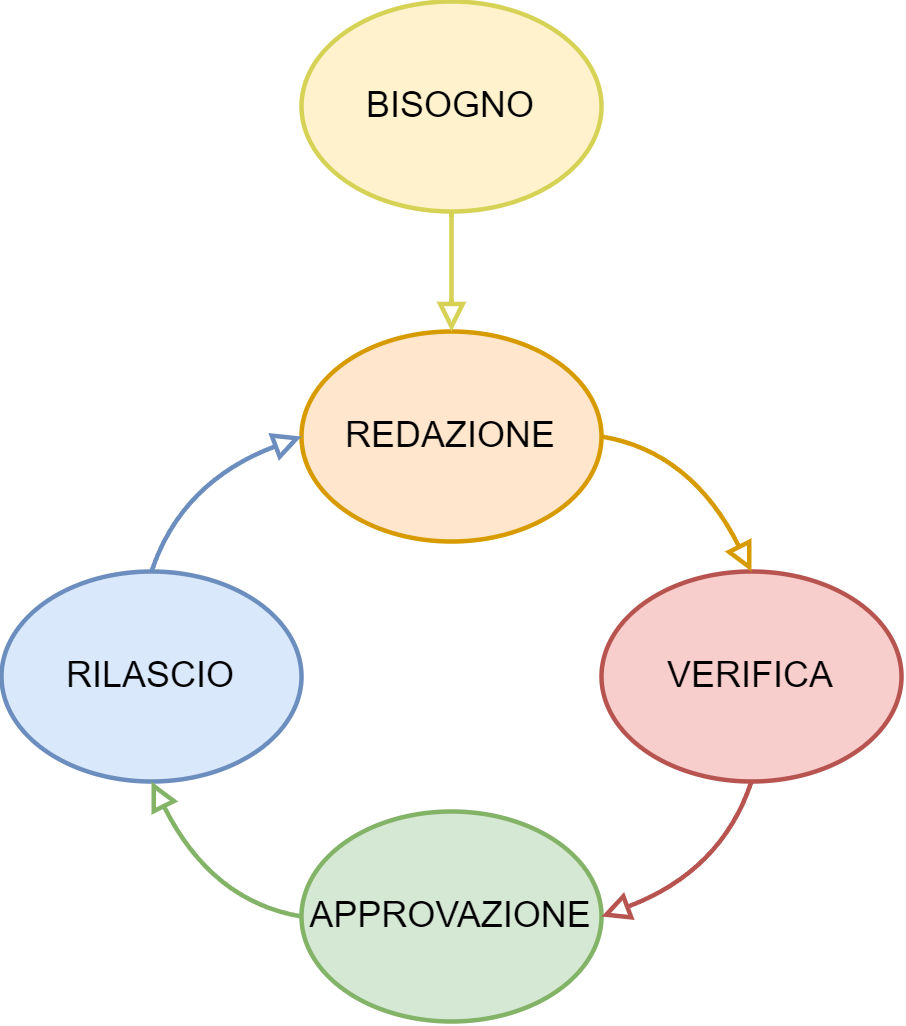
\includegraphics[scale=0.8]{doc_lifecycle.png}
    \caption{Ciclo di vita di un documento}
    \label{fig:doc_lifecycle}
\end{figure}
\subsubsection{Nome del file}
Il nome del file deve seguire la convenzione snake case\textsuperscript{G}, ovvero:
\begin{itemize}
    \item Ciascuna praola è scritta completamente in minuscolo
    \item Ogni parola è separata da un trattino basso `\_'
\end{itemize}
Inoltre, ciscun documento deve riportare, alla fine del nome, il codice di verione.
\par Ad esempio, per il documento sulle norme di progetto di versione 0.0.1 il nome del file deve essere:
\begin{center}
    norme\_di\_progetto\_v0.0.1
\end{center}
\subsubsection{Glossario}
Se il documento utilizza termini contenuti nel Glossario di progetto, quesi vanno segnalati nella sola prima istanza tramite la lettera \textbf{G} in apice, come da esempio:
\begin{center}
    termine\textsuperscript{G}
\end{center}
\subsubsection{Struttura del documento}
Il gruppo ha scelto di utilizzare una struttura fissa e prestabilita per la documentazione, allo scopo di rendere più efficienti la stesura, la verifica e la comprensione, che sono tutte facilitate nel caso in cui lo schema di regole da seguire sia unico e preciso.
\paragraph{Struttura generica}
Questa sezione descrive la struttura di un documento qualsiasi prodotto nel corso del progetto, esclusi i verbali, che per loro natura hanno bisogno di una struttura diversa.
\par Un documento (non verbale) si compone di quattro parti, qui elencate nell'ordine in cui devono comparire sul documento, separate tra loro da interruzioni di pagina.
\subparagraph{Intestazione.}
L'intestazione ha una struttura verticale che deve contenere, nell'ordine di esposizione, centrati orizzontalmente:
\begin{itemize}
    \item Logo
    \item Nome del gruppo
    \item Email del gruppo
    \item Titolo del documento
    \item Informazioni sul documento
    \begin{itemize}
        \item Versione
        \item Nome e cognome del responsabile interno che ha approvato il documento
        \item Nome e cognome di ciascun redattore
        \item Nome e cognome di ciascun verificatore
        \item Uso (interno o esterno)
    \end{itemize}
\end{itemize}
\subparagraph{Registro delle modifiche}
Il registro delle modifiche descrive le modifiche apportate al documento nel corso del tempo, dalla prima scrittura a quella attuale. Il registro è riportato nel documento in forma tabellare: dove ogni riga rappresenta una modifica e contiene:
\begin{itemize}
    \item Versione del documento
    \item Data di modifica
    \item Autore della modifica
    \item Ruolo dell'autore
    \item Descrizione della modifica
\end{itemize}
Le modifiche sono riportate, nell'ordine, dalla più vecchia alla più nuova.
\subparagraph{Indice dei contenuti.}
Questa sezione deve contenere un indice dei contenuti esposti nel documento, con i relativi numeri di pagina. Nel caso di documenti il cui contenuto è principalmente grafico (come l'analisi dei requisiti) o tabellare, sarà necessario inserire anche degli indici per le immagini o tabelle del documento.
\subparagraph{Argomenti.}
La sezione argomenti ha l'obiettivo di descrivere, gli argomenti discussi, le decisioni prese ed eventuali problematiche sorte nel corso dell'incontro. Per una comprensione più efficiente da parte del lettore, le descrizioni devono essere complete ma quanto più concise possibile.

\begin{center}
    \color{red}*** TODO ***
\end{center}
%Questa sezione descrive la struttura di un documento qualsiasi prodotto nel corso del progetto, esclusi i verbali, che per loro natura hanno bisogno di una struttura diversa.
%aggiunta dell'elenco figure o tabelle
\paragraph{Struttura di un verbale}
La struttura di un verbale ha una sezione dedicata perché, vista la differenza di informazioni che deve contenere, possiede una sua particolare struttura, diversa dagli altri documenti.
\par Un verbale si compone di cinque parti, qui elencate nell'ordine in cui devono comparire sul documento, separate tra loro da interruzioni di pagina.
\subparagraph{Intestazione.}
L'intestazione ha una struttura verticale che deve contenere, nell'ordine di esposizione, centrati orizzontalmente:
\begin{itemize}
    \item Logo
    \item Nome del gruppo
    \item Email del gruppo
    \item Titolo del documento
    \item Sottotitolo con obiettivo dell'incontro (nel solo caso di un verbale esterno)
    \item Informazioni sul documento
    \begin{itemize}
        \item Versione
        \item Nome e cognome del responsabile interno che ha approvato il documento
        \item Nome e cognome di ciascun redattore
        \item Nome e cognome di ciascun verificatore
        \item Uso (interno o esterno)
    \end{itemize}
\end{itemize}
\subparagraph{Registro delle modifiche e firma di approvazione.}
Il registro delle modifiche descrive le modifiche apportate al documento nel corso del tempo, dalla prima scrittura a quella attuale. Il registro è riportato nel documento in forma tabellare: dove ogni riga rappresenta una modifica e contiene:
\begin{itemize}
    \item Versione del documento
    \item Data di modifica
    \item Autore della modifica
    \item Ruolo dell'autore
    \item Descrizione della modifica
\end{itemize}
Le modifiche sono riportate, nell'ordine, dalla più vecchia alla più nuova.
\par Nonostante il verbale sia un documento che, per sua natura, richiede meno modifiche rispetto agli altri (che hanno uno sviluppo più incrementale), il gruppo ha scelto di inserirere un changelog per tenere traccia anche di eventuali richieste di modifica da parte dell'approvatore esterno prima della sua approvazione finale.
\par Alla fine del registro delle modifiche deve essere presente, nel solo caso dei verbali esterni, uno spazio per la firma di approvazione del partecipante esterno. Questa sezione deve contenere:
\begin{itemize}
    \item Versione del documento
    \item Data della firma
    \item Nome del firmatario
    \item Spazio per la firma
\end{itemize}
\subparagraph{Indice dei contenuti.}
Questa sezione deve contenere un indice dei contenuti esposti nelle due sezioni successive, con i relativi numeri di pagina.
\subparagraph{Informazioni.}
La sezione contiene le informazioni relative all'incontro descritto dal verbale. In particolare, deve riportare:
\begin{itemize}
    \item Informazioni di contesto
    \begin{itemize}
        \item Modalità: in presenza o da remoto (eventualmente su quale piattaforma)
        \item Data dell'incontro
        \item Orario di inizio e orario di fine
    \end{itemize}
    \item Partecipanti
    \begin{itemize}
        \item Interni, suddivisi tra presenti e assenti
        \item Esterni
    \end{itemize}
\end{itemize}
Se per l'incontro il gruppo ha selezionato un portavoce, questo deve essere segnato vicino al suo nome nell'elenco dei presenti.
\subparagraph{Argomenti.}
La sezione argomenti ha l'obiettivo di descrivere, gli argomenti discussi, le decisioni prese ed eventuali problematiche sorte nel corso dell'incontro. Per una comprensione più efficiente da parte del lettore, le descrizioni devono essere complete ma quanto più concise possibile.
\subsubsection{Template}
Al fine di mantenere una struttura quanto più coerente possibile e di velocizzare la scrittura della documentazione, il gruppo ha costruito un template per ciascun tipo di documento (verbale o generico), sul quale il redattore si deve basare per stilare un nuovo documento. 
\subsubsection{Strumenti}
\paragraph{\LaTeX}
Per la scrittura dei documenti il gruppo ha scelto di utilizzare \LaTeX, un linguaggio di marcatura creato appositamente per la preparazione di testi, basato sul programma per la tipografia digitale \TeX. Lo strumento facilita la stesura di un documento perché molti aspetti, quali ad esempio la numerazione delle sezioni, delle pagine e l'indice dei contenuti, vengono gestiti in maniera automatica, permettendo al redattore di focalizzarsi sul contenuto e lavorare in maniera più efficiente. Inoltre, è possibile lavorare su file diversi e unirli per costruire un singolo documento, facilitando la collaborazione tra membri del gruppo.
\par Lo strumento è reperibile al sito:
\begin{center}
    \url{https://www.latex-project.org/}
\end{center}
\paragraph{Visual Studio Code}
Visual Studio Code è un editor di codice sorgente libero, gratuito e leggero che permette, tramite l'utilizzo del plugin ``LaTeX workshop", un utilizzo veloce del linguaggio \LaTeX, fornendo strumenti come l'autocompletamento, la segnalazione di errori e la compilazione del documento in formato PDF.
\par Lo strumento è reperibile al sito:
\begin{center}
    \url{https://code.visualstudio.com/}
\end{center}
\paragraph{Diagrams.net}
Per la costruzione di diagrammi, in particolare per i diagrammi UML, il gruppo utilizza diagrams.net, una piattaforma gratuita per il disegno di grafi, che fornisce supporto a diverse tipologie di diagrammi, selezionata per la sua interfaccia semplice ed intuitiva e per la possibilità di salvare gli schemi prodotti in molti formati.
\par Lo strumento è reperibile al sito:
\begin{center}
    \url{https://www.drawio.com/}
\end{center}

%%%%%%%%%%%%%%%%%%%%%%%%%%%%%%%%%%%
%%% GESTIONE DELLA CONFIGURAZIONE
%%%%%%%%%%%%%%%%%%%%%%%%%%%%%%%%%%%
\subsection{Gestione della configurazione}\label{sec:processi_di_supporto:gestione_configurazione}
La gestione della configurazione è l'attività dello sviluppo software che si occupa della gestione e controllo dei software items\textsuperscript{G}, in particolare della documentazione e del codice prodotto, nel corso del progetto.
\par È un processo particolarmente importante: permette di tracciare le modifiche nel tempo, migliora la collaborazione attraverso la condivisione dei file ed assicura una maggiore affidabilità del sistema, perché facilita l'individuazione e la risoluzione di errori.
\subsubsection{Versionamento}
Per poter identificare una particolare istanza di un software item in uno specifico momento temporale e differenziarla dalle altre, il gruppo ha scelto di assegnare un codice di versionamento a ciscun item che si preveda possa subire modifiche ed evolvere nel corso del progetto. Il codice utilizza cifre numeriche ed è scritto come segue:
\begin{center}
    \textbf{[X].[Y].[Z]}
\end{center}
Dove \textbf{X}, \textbf{Y} e \textbf{Z} sono numeri interi tali che:
\begin{itemize}
    \item \textbf{X}: è un numero $ \geq 0 $ che aumenta ad ogni approvazione del responsabile interno
    \item \textbf{Y}: è un numero $ \geq 0 $ che aumenta ad ogni controllo del verificatore
    \item \textbf{Z}: è un numero $ \geq 0 $ che aumenta ad ogni modifica del redattore
    \item Se \textbf{Y} aumenta di 1, allora \textbf{Z} torna al valore 0
    \item Se \textbf{X} aumenta di 1, allora sia \textbf{Y} che \textbf{Z} tornano al valore 0
\end{itemize}
Ciascun software item inizia dalla versione \textbf{0.0.1} e prosegue come descritto.
\subsubsection{Strumenti}
\paragraph{Git}
Lo strumento principale utilizzato per questo processo è Git, un software per il controllo di versione con interfaccia a riga di comando. Si tratta di uno strumento molto famoso ed estremamente utilizzato, progettato per avere alte prestazioni e per garantire l'integrità dei file che gestisce: per queste ragioni, è considerato lo standard \textit{de facto} nell'ambito dei version control systems.
\par Lo strumento è reperibile al sito:
\begin{center}
    \url{https://git-scm.com/}
\end{center}
\paragraph{Gitflow}
Altra caratteristica importante di Git è la sua flessibilità di utilizzo: infatti, esistono diverse strategie di utilizzo per questo strumento, definite workflows, il cui obiettivo è stabilire delle linee guida per utilizzare Git in maniera consistente e produttiva.
\par Il workflow che il gruppo ha deciso di adottare è Gitflow, che suggerisce di assegnare ruoli specifici ai diversi branch e definisce le modalità secondo cui devono interagire.
\par Nello specifico, l'adozione del Gitflow workflow comporta la creazione di quattro tipologie di branch:
\begin{itemize}
    \item \textbf{Main}: è il ramo principale, sul quale si trova l'ultima versione funzionante e rilasciata del prodotto. Non si lavora mai direttamente sul ramo principale, per lasciarne intatto il contenuto
    \item \textbf{Release}: è il ramo in cui si lavora per fare le ultime operazioni prima di un rilascio: una volta che tutto è pronto, il suo contenuto viene passato al main e rappresenta ufficialmente una nuova versione
    \item \textbf{Develop}: è il ramo su cui si lavora principalmente, contiene il prodotto incompleto e in fase di lavorazione. Quando lo sviluppo raggiunge una fase tale per cui il prodotto è pronto per il rilascio, si passa il contenuto nel ramo release per gli ultimi ritocchi.
    \item \textbf{Feature}: ogni ramo feature si stacca dal develop e serve per lavorare separatemente su una specifica feature del prodotto (una parte di codice oppure un documento), in modo tale che il ramo develop non subisca alterazioni mentre la feature è in fase di lavorazione.
\end{itemize}
In particolare, un aspetto importante di questo workflow è la separazione dei lavori: infatti, permette a ciascun utente di lavorare sul progetto senza bloccare gli altri, perché si lavora su rami feature separati e, in ogni caso, non si lavora sul main, che quindi contiene sempre un prodotto funzionante e completo.
\par Maggiori informazioni sono presenti alla sezione \ref{sec:riferimenti_esterni:materiali_di_studio}, che contiene documentazione e tutorial sugli strumenti di progetto.


\subsection{Accertamento della qualità}\label{sec:processi_di_supporto:accertamento_qualità}

\begin{center}
    \color{red}*** TODO ***
\end{center}

\subsection{Verifica}\label{sec:processi_di_supporto:verifica}

\begin{center}
    \color{red}*** TODO ***
\end{center}

\subsection{Validazione}\label{sec:processi_di_supporto:validazione}

\begin{center}
    \color{red}*** TODO ***
\end{center}


\newpage
%%%%%%%%%%%%%%%%%%%%%%%%%%%%%%%%%%%
% PROCESSI ORGANIZZATIVI
%%%%%%%%%%%%%%%%%%%%%%%%%%%%%%%%%%%
\section{Processi organizzativi}\label{sec:processi_organizzativi}
%\subsection{Gestione dei processi}\label{sec:processi_organizzativi:gestione_processi}
%Questo processo riguarda le attività di carattere gestionale ed organizzativo che il gruppo deve svolgere per gestire gli altri processi nel corso del progetto. Sostanzialmente, descrive il coordinamento tra membri del gruppo e gli obiettivi che ciascuno deve raggiungere.
%\subsubsection{Way of working}
%Per facilitare il corretto utilizzo delle procedure e degli strumenti, il gruppo deve delineare il proprio way of working e descriverlo formalmente in un documento, consultabile da ciascun membro in qualsiasi momento. Il documento di riferimento è ``Norme di progetto", che deve essere redatto in maniera incrementale, aggiornando le procedure, le convenzioni e gli strumenti utilizzati durante il corso del progetto.

\begin{center}
    \color{red}*** TODO ***
\end{center}

\subsection{Gestione delle infrastrutture}\label{sec:processi_organizzativi:gestione_infrastrutture}

\begin{center}
    \color{red}*** TODO ***
\end{center}

\subsection{Formazione del personale}\label{sec:processi_organizzativi:formazione_personale}
Lo sviluppo di un progetto dipende notevolmente dalle abilità e dalle conoscenze del team: se i componenti sanno utilizzare gli strumenti e conoscono l'argomento del progetto, allora saranno in grado di realizzare un prodotto di qualità, più efficace ed efficiente e con tempi di lavoro ridotti.
\subsubsection{Modalità di formazione}
La materia di interesse, la programmazione 3D, è un argomento che i membri del gruppo non hanno avuto modo di approfondire nel loro percorso formativo, così come gli strumenti adottati.
\par Per questi motivi, il gruppo si impegna a mantenere un processo di formazione autonoma ed individuale durante il corso del progetto e a definire una serie di procedure ed automatismi (dove possibile), allo scopo di lavorare sfruttando interamente le opportunità che gli strumenti offrono, per poter soddisfare pienamente le aspettative del commitente e del proponente.
\par I materiali di studio suggeriti possono essere consultati nella sezione \ref{sec:riferimenti_esterni:materiali_di_studio}, che riporta i riferimenti esterni alla documentazione e tutorial per gli strumenti e le tecnologie utilizzati nel progetto.

\newpage
%%%%%%%%%%%%%%%%%%%%%%%%%%%%%%%%%%%
% STANDARD ISO/IEC 12207
%%%%%%%%%%%%%%%%%%%%%%%%%%%%%%%%%%%
\newpage
\section{Standard ISO/IEC 12207}\label{sec:standard_iso/iec_12207}
ISO/IEC 12207 è uno standard internazionale nato con l'obiettivo di diventare il riferimento primario per la gestione del ciclo di vita\textsuperscript{G} del software: in effetti, è il modello più utilizzato e conosciuto, perciò rappresenta una buona garanzia di successo se applicato correttamente nello sviluppo software.
\par Si tratta di uno standard più descrittivo che tecnico: infatti, riconosce la possibilità che il ciclo di sviluppo possa variare a seconda delle necessità e perciò non definisce un approccio specifico, ma piuttosto delinea una serie di processi che il ciclo deve attraversare, in una struttura modulare e flessibile per permettere agli utilizzatori di adattarlo alle proprie esigenze.
\par Lo standard suddivide i processi in tre categorie: processi \textbf{primari} (o \textbf{base}), processi di \textbf{supporto} e processi \textbf{organizzativi}, qui descritti in maniera sommaria per permettere al lettore una migliore comprensione della struttura del documento. Per una lettura più approfondita e rigorosa, si rimanda alla sezione \hyperref[sec:riferimenti_esterni]{Riferimenti Esterni}, che contiene un link alla versione originale (1995) dello standard.

%%%%%%%%%%%%%%%%%%%%%%%%%%%%%%%%%%%
%%% PROCESSI PRIMARI
%%%%%%%%%%%%%%%%%%%%%%%%%%%%%%%%%%%
\subsection{Processi primari}
Sono cinque processi a stretto contatto con lo sviluppo software che servono ai principali soggetti coinvolti nel suo ciclo di vita.
\subsubsection{Acquisizione}
Descrive le attività e gli obiettivi dell'acquirente, cioè di quel soggetto che identifica un'opportunità: ha il bisogno di acquisire un sistema, prodotto o servizio software, seleziona un fornitore e decide se accettare o meno tale sistema, prodotto o servizio proposto dal fornitore.
\par Le sottoattività in cui si suddivide questo processo sono infatti:
\begin{itemize}
    \item Acquisition preparation
    \item Supplier selection
    \item Supplier monitoring
    \item Customer acceptance
\end{itemize}
\subsubsection{Fornitura}
Questo processo, che delinea i compiti del fornitore, ha inizio nel momento in cui questo decide di produrre una proposta per rispondere alle richieste di un acquirente oppure quando firma un contratto con l'acquirente per lo sviluppo di un sistema, prodotto o servizio software. In particolare, il processo comprende la selezione di procedure e risorse necessarie a completare il progetto e la gestione dei rapporti con il cliente.
\par Il processo si suddivide nelle seguenti sottoattività:
\begin{itemize}
    \item Supplier tendering
    \item Contract agreement
    \item Product release
    \item Product acceptance support
\end{itemize}
\subsubsection{Sviluppo}
Contiene tutte le attività e gli obiettivi dello sviluppatore, dall'analisi dei requisiti, al design, alla programmazione con testing, fino all'installazione del prodotto, che deve soddisfare le richieste di contratto stipulate con il cliente.
\par Più nello specifico, il processo si suddivide in diverse sottoattività:
\begin{itemize}
    \item Requirements elicitation
    \item System requirements analysis
    \item System architectural design
    \item Software requirements analysis
    \item Software architectural design
    \item Software detailed design
    \item Software coding and testing
    \item Software integration
    \item Software qualification testing
    \item System integration
    \item System qualification testing
    \item Software installation
\end{itemize}
\subsubsection{Gestione operativa}
Il processo riguarda l'installazione ed erogazione del prodotto software, con riferimento anche al sistema nel quale il prodotto opera e al supporto per gli utenti utilizzatori.
\par Si suddivide in:
\begin{itemize}
    \item Operational use
    \item Customer acceptance
\end{itemize}
\subsubsection{Manutenzione}
Il processo si attiva quando il prodotto software deve essere modificato nel codice e di conseguenza nella documentazione associata, per risolvere difetti oppure per apportare miglioramenti o adattamenti a seconda delle necessità e ha come obiettivo quello di modificare il prodotto, mantenendo la sua integrità. Il processo include la migrazione e il ritiro del prodotto e, di fatto, si conclude proprio con quest'ultima fase.

%%%%%%%%%%%%%%%%%%%%%%%%%%%%%%%%%%%
%%% PROCESSI DI SUPPORTO
%%%%%%%%%%%%%%%%%%%%%%%%%%%%%%%%%%%
\subsection{Processi di supporto}
Sono otto processi, ciascuno con un suo obiettivo ben definito che, come il nome suggerisce, supportano altri processi e possono essere utilizzati da questi ogni volta che lo ritengano necessario.

\subsubsection{Documentazione}
Il processo di documentazione si occupa di registrare le informazioni prodotte dai processi durante il ciclo di vita del prodotto e delinea un elenco di attività che seguono la redazione di un documento nelle sue diverse fasi: dalla pianificazione e progettazione, alla scrittura e modifica, fino alla distribuzione e manutenzione.
\subsubsection{Gestione della configurazione}
Applica procedure tecniche e di amministrazione durante il ciclo di vita software con l'obiettivo di identificare i diversi software items, registrare il loro stato nel tempo e gestirne le modifiche ed i rilasci.
\subsubsection{Accertamento della qualità}
Si occupa di accertarsi che il software in produzione sia conforme agli specifici requisiti richiesti dal cliente e che rispetti i piani e gli standard prestabiliti. Può fare uso di altri processi di supporto, come verifica e validazione, revisione con il cliente, verifiche interne e risoluzione dei problemi.
\subsubsection{Verifica}
Ha l'obiettivo di determinare se le attività compiute durante il corso del progetto sono conformi alle specifiche decise nelle attività precedenti. Nella fase di sviluppo, ad esempio, la verifica spesso consiste nell'esecuzione ripetuta di test su porzioni più o meno grandi del codice (ma anche sul prodotto nella sua interezza) per capire se il programma si sta comportando in maniera coerente con quanto stabilito nella fase di design.
\par È consigliabile che questo processo abbia inizio quanto prima possibile nei processi primari che lo includono.
\subsubsection{Validazione}
La validazione ha il compito di accertarsi che le attività di progetto risultino in un prodotto finale che rispetti i requisiti preposti dal cliente e soddisfi i bisogni originali per i quali il progetto ha avuto origine.
\subsubsection{Revisione congiunta con il cliente}
Questo processo nasce per valutare assieme agli stakeholders lo stato e gli output delle diverse attività di progetto, per accertarsi che rispettino gli accordi prestabiliti e per decidere come intervenire in caso contrario.
\par Può essere impiegato sia a livello di gestione del progetto che a livello tecnico, perferibilmente durante tutto il corso del progetto.
\subsubsection{Verifiche ispettive interne}
Conosciuto anche come \textit{audit}, è un processo di revisione nel quale uno o più soggetti (detti \textit{auditors}) si accertano che il software sia conforme agli standard, ai requisiti e al contratto con il cliente.
\par Per tutelare il cliente ed ottenere una revisione imparziale, è necessario che gli auditors non siano direttamente responsabili del prodotto che stanno esaminando.
\subsubsection{Risoluzione dei problemi}
Ha lo scopo di analizzare e risolvere i problemi di qualunque natura che possono sorgere durante l'esecuzione di altri processi (in particolare, i processi di sviluppo, gestione operativa e manutenzione), con l'obiettivo di intervenire velocemente ed in maniera responsabile.
\par È importante anche documentare qualsiasi tipo di problematica per poterle poi classificare per categoria e per individuare certi tipi di pattern.

%%%%%%%%%%%%%%%%%%%%%%%%%%%%%%%%%%%
%%% PROCESSI ORGANIZZATIVI
%%%%%%%%%%%%%%%%%%%%%%%%%%%%%%%%%%%
\subsection{Processi organizzativi}
Sono quattro processi trasversali che non riguardano lo specifico progetto, ma l'aspetto di management e dovrebbero essere impiegati dall'organizzazione per migliorare la propria struttura e coordinazione.
\subsubsection{Gestione dei processi}
Contiene tutta una serie di obiettivi ed attività di carattere gestionale che possono essere impiegate da qualsiasi soggetto coinvolto per gestire i propri processi. In particolare, si suddividono in attività di:
\begin{itemize}
    \item Pianificazione: per ciascun processo, bisogna stabilire i lavori da svolgere, stimare il tempo necessario a concluderli, determinare le risorse necessarie e i costi, assegnare i ruoli e le responsabilità
    \item Esecuzione e controllo: per mettere in atto il piano stabilito e monitorare l'andamento del processo, per assicurarsi che tutto proceda secondo i piani.
    \item Revisione: nella quale ci si assicura che il prodotto e i piani soddisfino i requisiti preposti, valutando anche l'andamento del processo rispetto alla pianificazione iniziale.
\end{itemize}
\subsubsection{Gestione delle infrastrutture}
Il processo ha il compito di stabilire e mentenere attiva l'infrastruttura necessaria per gli altri processi. Tale infrastruttura può essere di carattere sia software che hardware, ma può riguardare anche strumenti, tecniche e standard.
\subsubsection{Miglioramento del processo}
Si occupa di effettuare misure e controlli per stabilire e migliorare i processi di ciclo di vita del software.
\subsubsection{Formazione del personale}
Dato che la buona riuscita di tutti i processi (in particolare quelli primari) dipende dalle abilità e conoscenze del personale, questo processo si occupa di accertarsi che il personale abbia una formazione adeguata per i compiti che si trova a svolgere durante il corso del progetto.

\newpage
%%%%%%%%%%%%%%%%%%%%%%%%%%%%%%%%%%%
% RIFERIMENTI ESTERNI
%%%%%%%%%%%%%%%%%%%%%%%%%%%%%%%%%%%
\newpage
\section{Riferimenti esterni}\label{sec:riferimenti_esterni}
Per ulteriori chiarimenti sugli argomenti discussi nel documento, si possono consultare i seguenti link esterni:
\begin{itemize}
    \item Capitolato \textbf{Warehouse Management 3D}:\\
    \url{https://www.math.unipd.it/~tullio/IS-1/2023/Progetto/C5.pdf}
    \item \textbf{Regolamento} del progetto didattico:\\
    \url{https://www.math.unipd.it/~tullio/IS-1/2023/Dispense/PD2.pdf}
    \item Link alla \textbf{documentazione del gruppo}:\\
    \url{https://avant-garde-software-engineering.github.io/documentazione.html}
    \item Standard \textbf{ISO/IEC 12207}, versione 1995:\\
    \url{https://www.math.unipd.it/~tullio/IS-1/2009/Approfondimenti/ISO_12207-1995.pdf}
    \item Link alle \textbf{slides sui processi del ciclo di vita}, con sottoattività per i processi dello standard ISO/IEC 12207:\\
    \url{https://www.math.unipd.it/~tullio/IS-1/2023/Dispense/T2.pdf}
\end{itemize}
\subsection{Materiali di studio}\label{sec:riferimenti_esterni:materiali_di_studio}
\subsubsection{Documentazione}
\begin{itemize}
        \item \LaTeX: \url{https://www.latex-project.org/help/documentation/}
        \item Visual Studio Code: \url{https://code.visualstudio.com/docs}
        \item Diagrams.net: \url{https://www.drawio.com/doc/#get-started-with-diagramsnet}
        \item Git: \url{https://git-scm.com/doc}
        \item Github: \url{https://docs.github.com/en}
    \end{itemize}
\subsubsection{Tutorial}
\begin{itemize}
        \item Gitflow:
            \begin{itemize}
                \item \url{https://www.atlassian.com/git/tutorials/comparing-workflows/gitflow-workflow}
                \item \url{https://danielkummer.github.io/git-flow-cheatsheet/}
            \end{itemize}       
                        
    \end{itemize}